\section{Исследовательская часть}

В данном разделе будут приведены примеры работы программ и сравнительный анализ алгоритмов на основе полученных данных.

\subsection{Технические характеристики}

Технические характеристики устройства, на котором выполнялись замеры времени:
\begin{itemize}
    \item Процессор: \texttt{AMD Ryzen™ 7 4700U} 2.0 ГГц \cite{amd}, 8 физических ядер, 8 потоков;
    \item Оперативная память: 8 ГБ, \texttt{DDR4}, 3200 МГц;
    \item Операционная система: \texttt{NixOS 23.05.4448.5550a} \cite{nixos};
    \item Версия ядра: \texttt{6.1.59}.
\end{itemize}

\subsection{Демонстрация работы программы}

На рисунках \ref{fig:demo1} -- \ref{fig:demo3} представлена демонстрация работы программы: ручной ввод слов, проведение замеров времени и постровение графиков.

\begin{figure}[H]
	\centering
	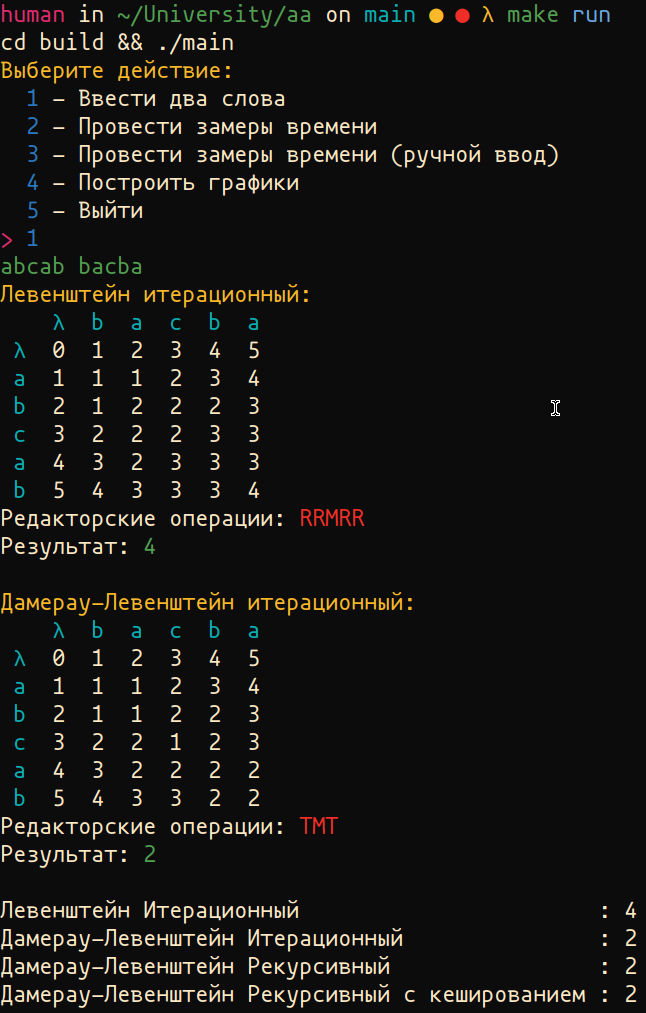
\includegraphics[scale=0.7]{img/demo1.png}
	\caption{Демонстрация работы программы, ввод двух слов}
	\label{fig:demo1}
\end{figure}

\begin{figure}[H]
	\centering
	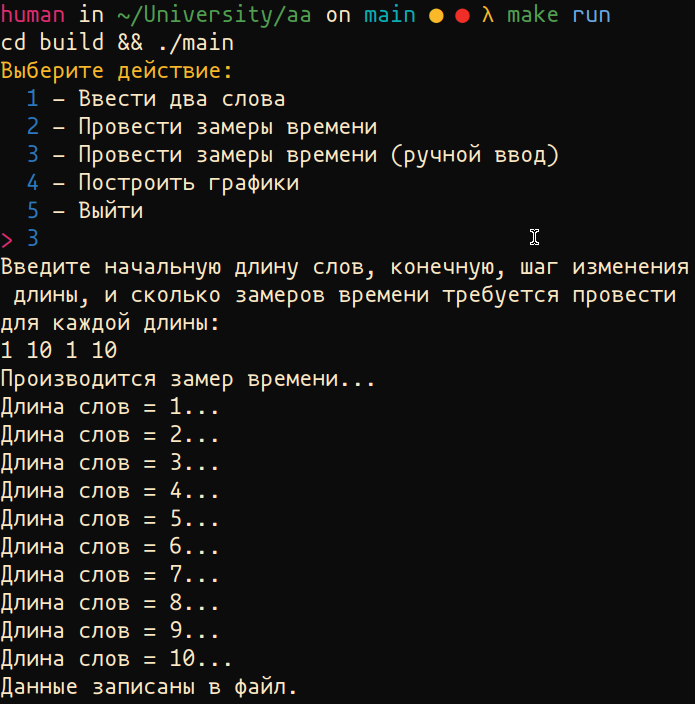
\includegraphics[scale=0.7]{img/demo2.png}
	\caption{Демонстрация работы программы, проведение замеров времени}
	\label{fig:demo2}
\end{figure}

\begin{figure}[H]
	\centering
	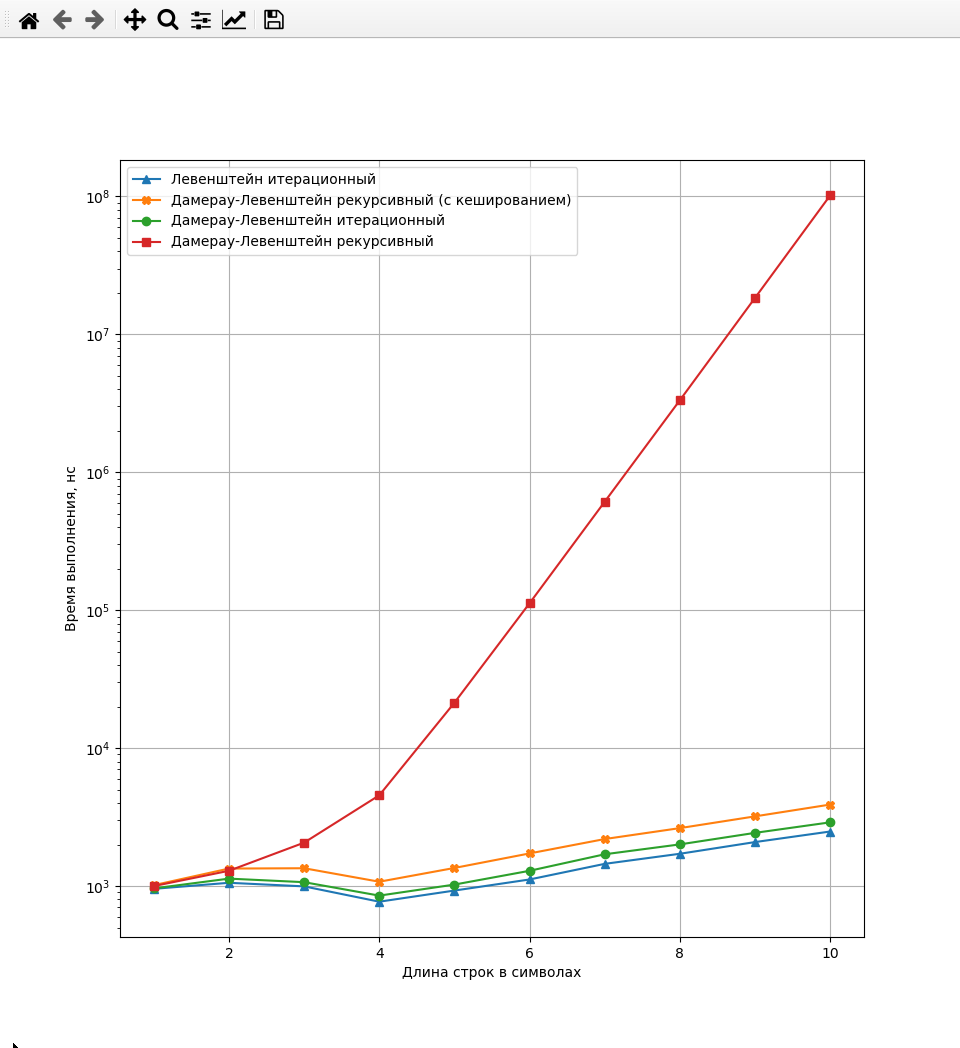
\includegraphics[scale=0.5]{img/demo3.png}
	\caption{Демонстрация работы программы, построение графиков на основе последних замеров времени (создаётся дочерний процесс, который запускает \texttt{Python}-скрипт)}
	\label{fig:demo3}
\end{figure}

\newpage

\subsection{Временные характеристики}

На графиках \ref{fig:fn_iter} -- \ref{fig:fn_four} представлены результаты замеров времени выполнения реализаций алгоритмов нахождения расстояний Левенштейна и Дамерау~---~Левенштейна.
Замеры времени проводились для строк одинаковой длины.
Отображённое на графиках время является усреднённым для каждой длины строк.

\begin{figure}[H]
	\centering
	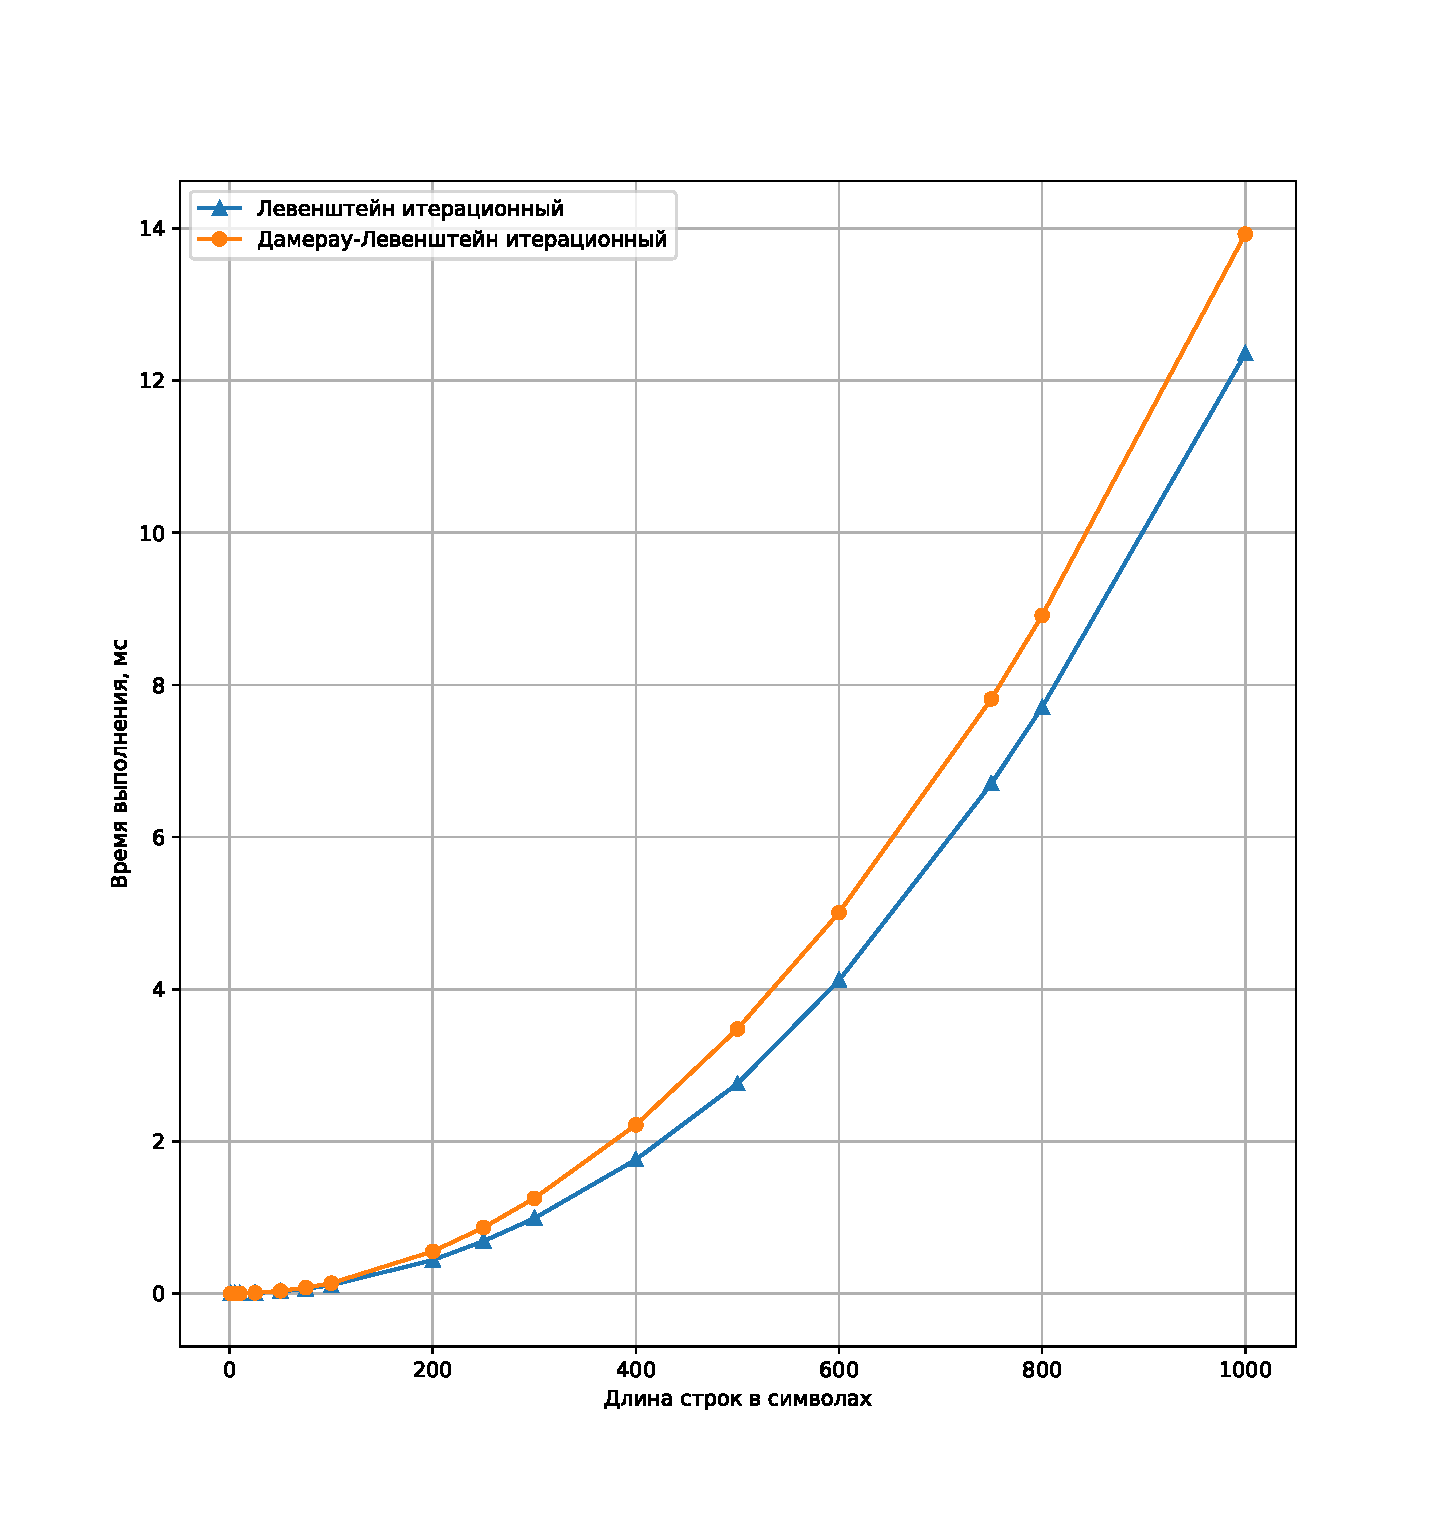
\includegraphics[width=\textwidth]{img/fn_iter.pdf}
	\caption{Сравнение реализаций итерационных алгоритмов по времени выполнения (среднее время из 100 замеров)}
	\label{fig:fn_iter}
\end{figure}

\begin{figure}[H]
	\centering
	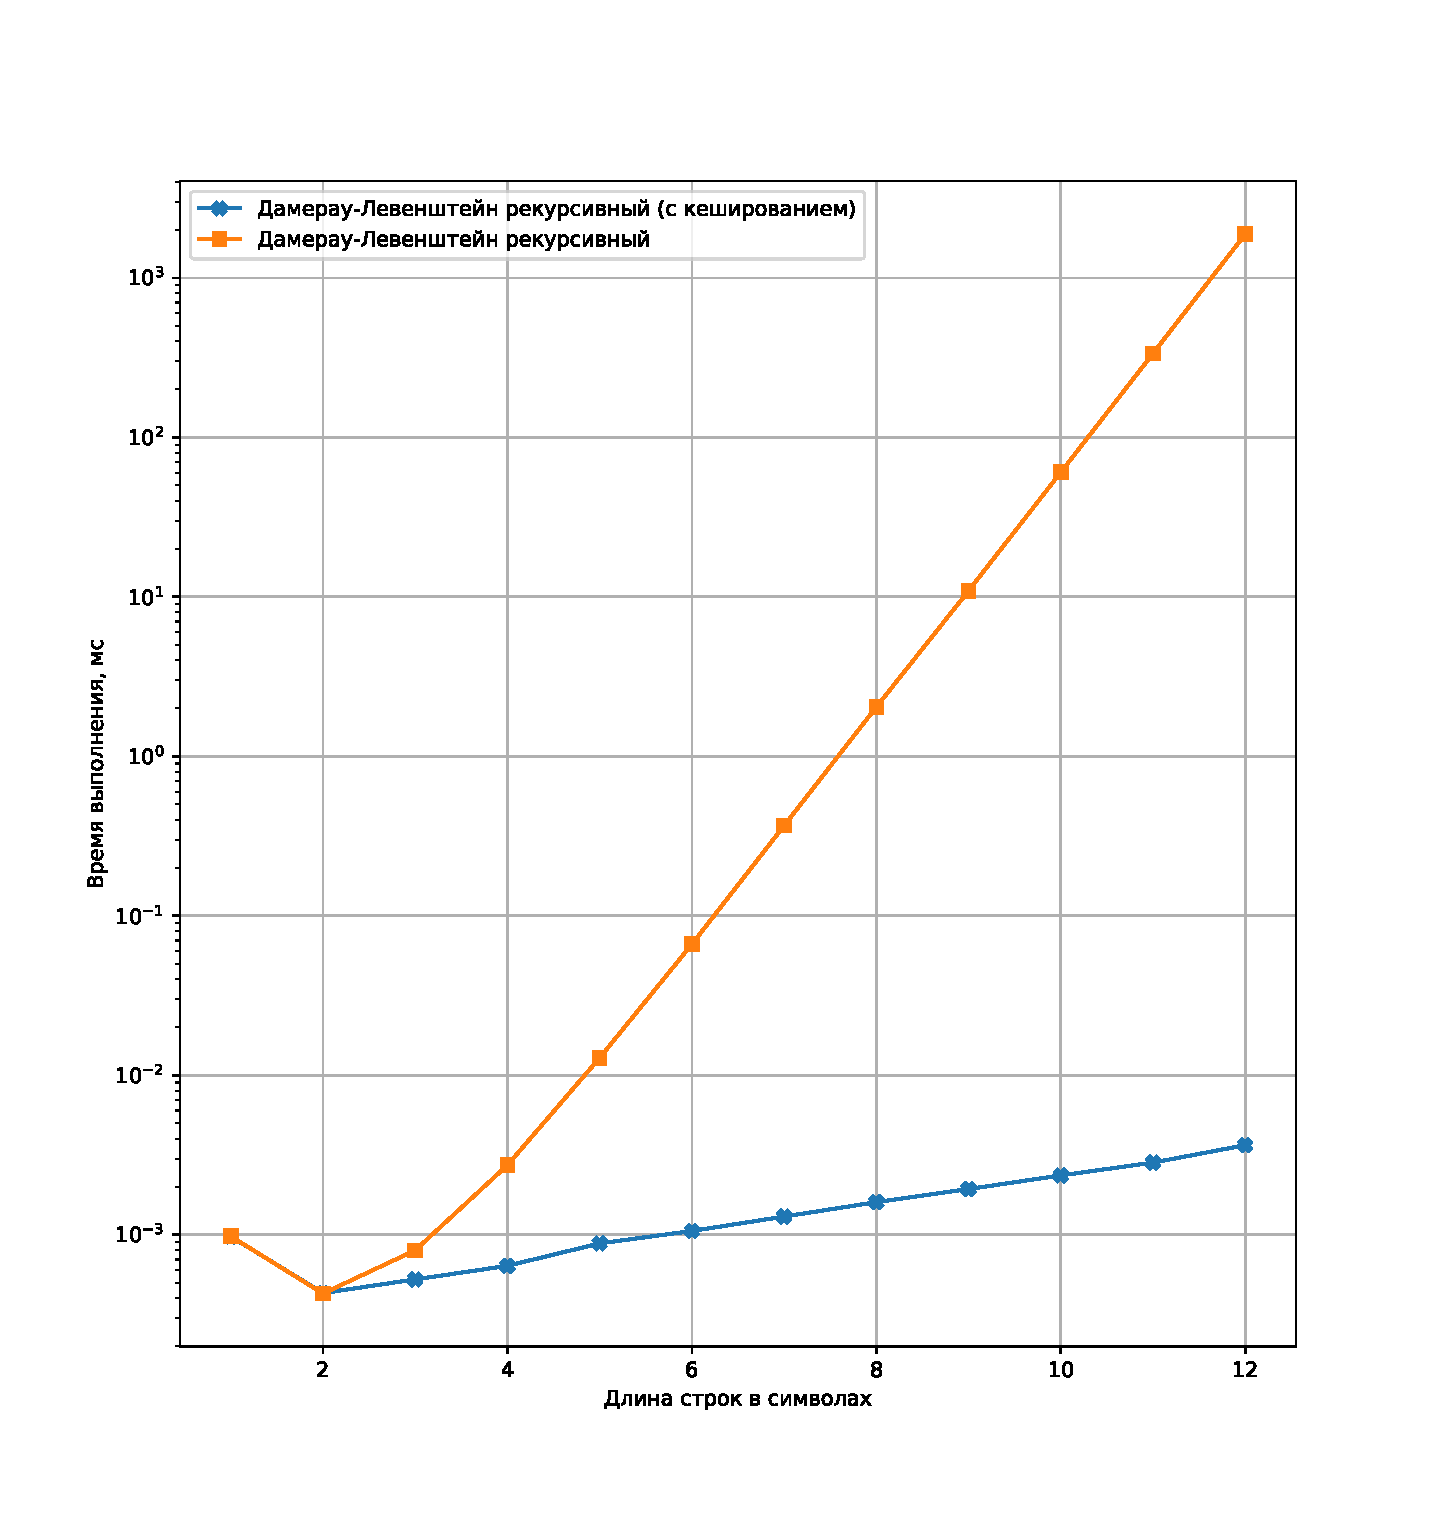
\includegraphics[width=\textwidth]{img/fn_rec.pdf}
	\caption{Сравнение реализаций рекурсивных алгоритмов по времени выполнения (среднее время из 10 замеров)}
	\label{fig:fn_rec}
\end{figure}

\begin{figure}[H]
	\centering
	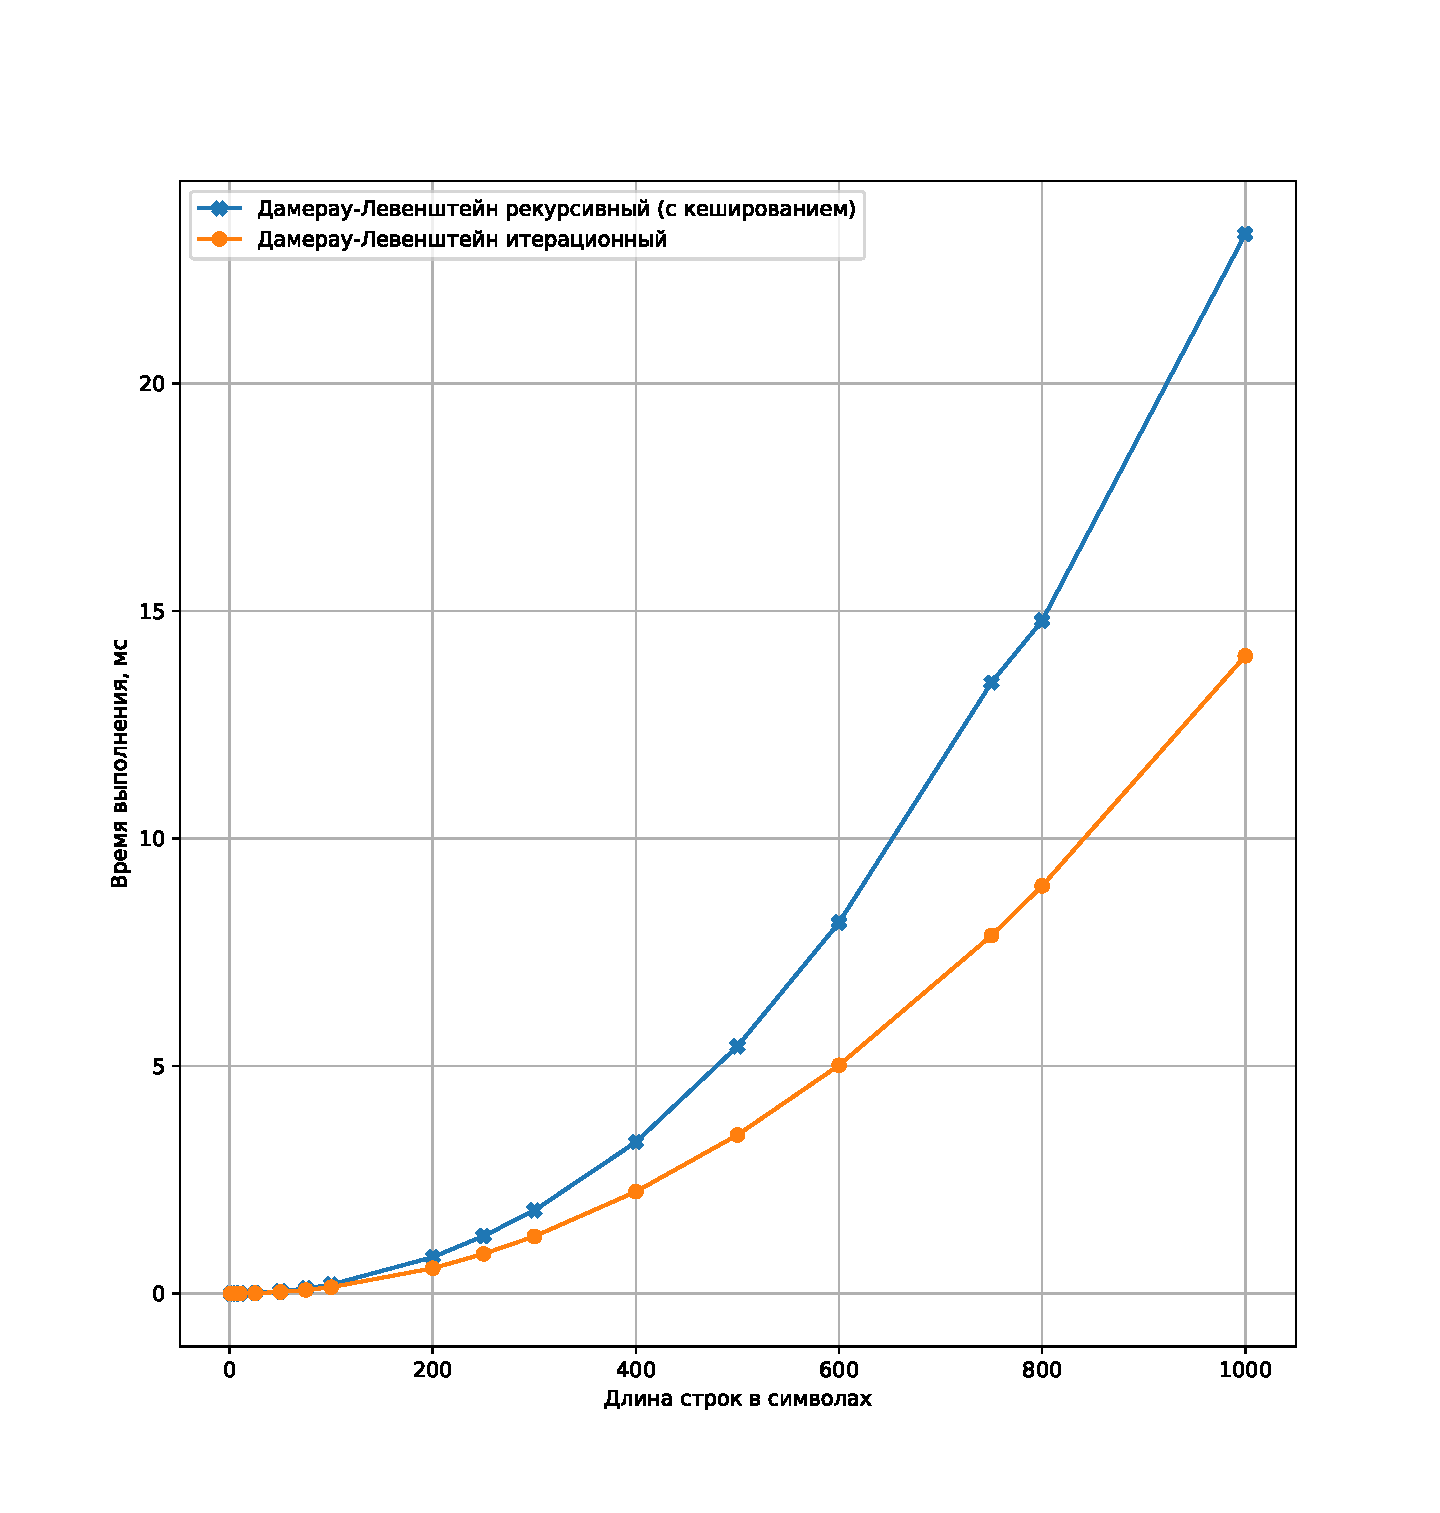
\includegraphics[width=\textwidth]{img/fn_damlev_iter_rec.pdf}
	\caption{Сравнение итерационной и рекурсивной с кешированием реализации алгоритмов нахождения расстояния Дамерау --- Левенштейна по времени выполнения (среднее время из 100 замеров)}
	\label{fig:fn_dlir}
\end{figure}

\begin{figure}[H]
	\centering
	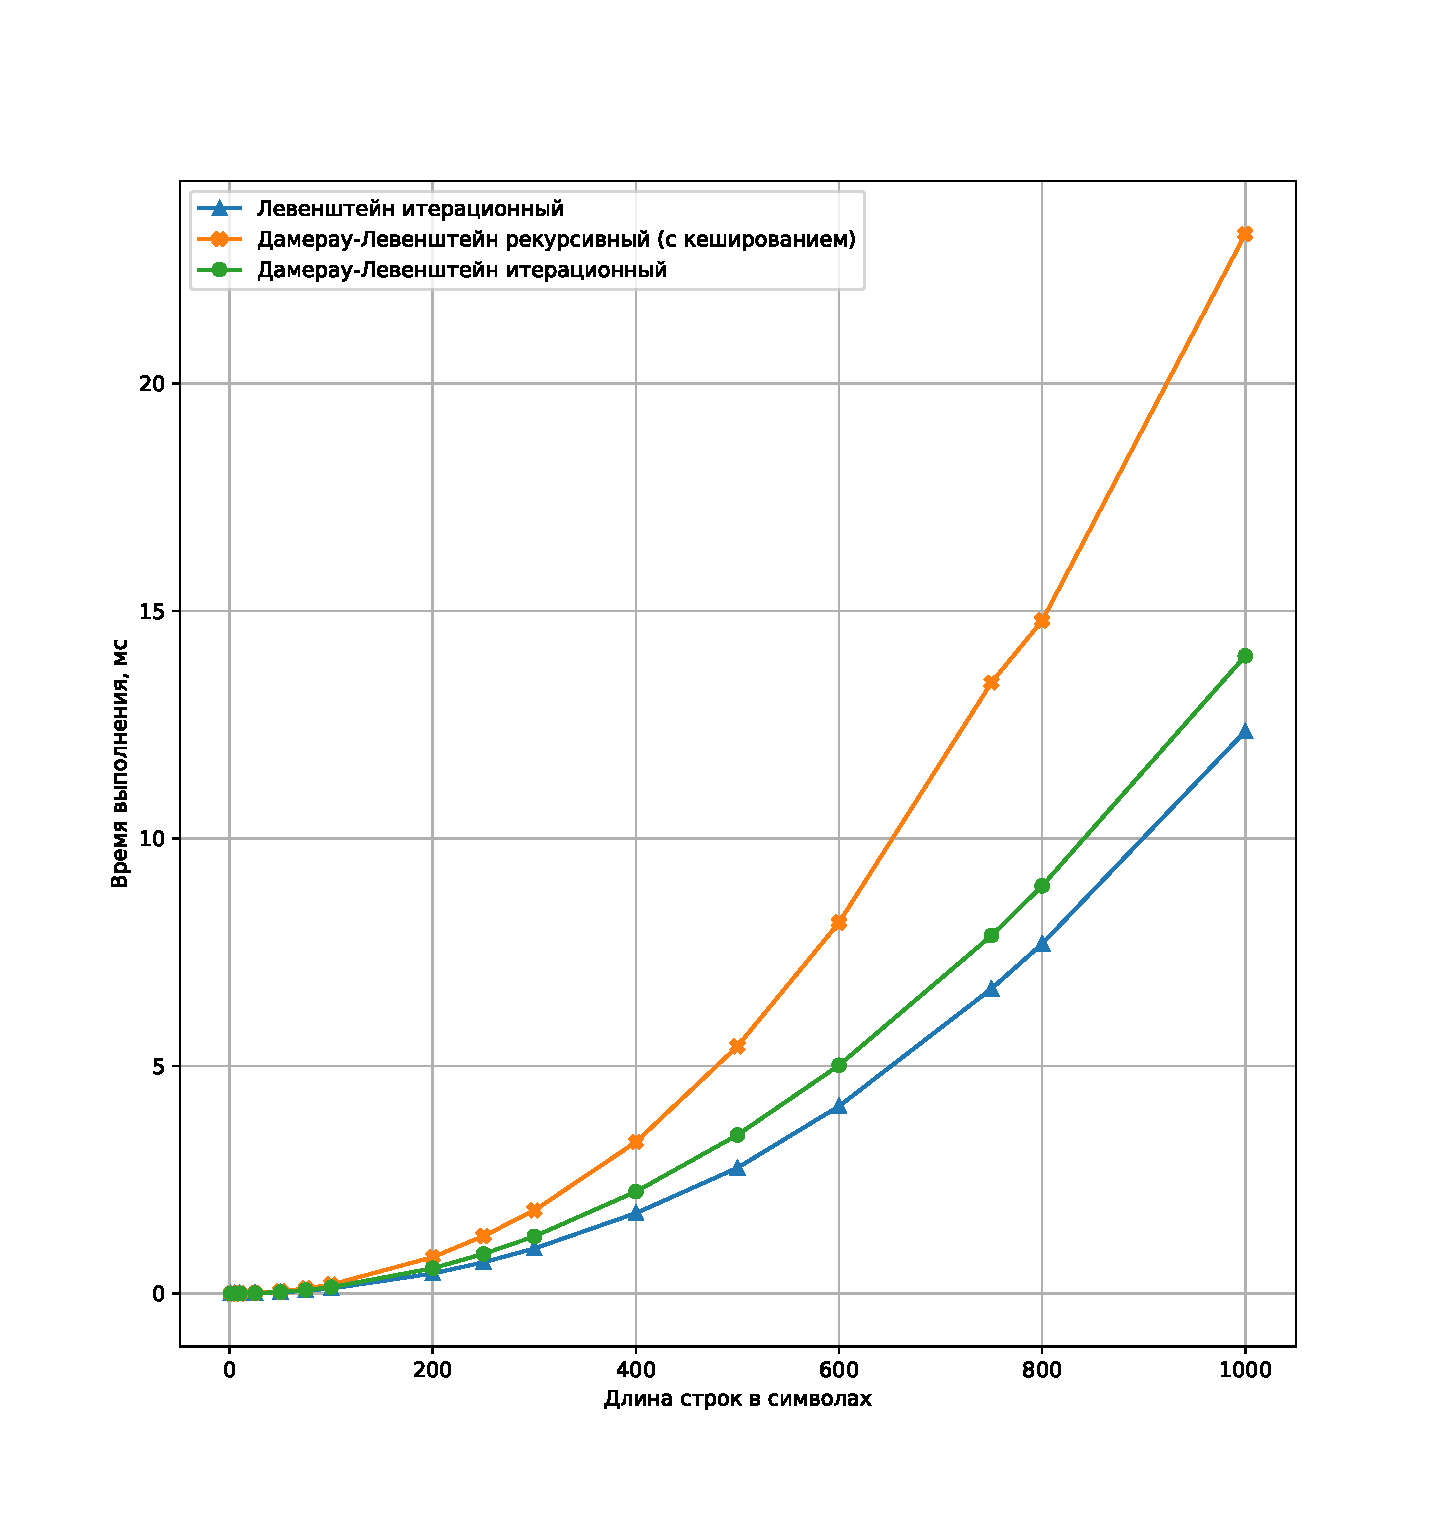
\includegraphics[width=\textwidth]{img/fn_three.pdf}
	\caption{Сравнение итерационных и рекурсивной с кешированием реализаций алгоритмов нахождения расстояний Левенштейна и Дамерау~---~Левенштейна по времени выполнения (среднее время из 100 замеров)}
	\label{fig:fn_three}
\end{figure}

\begin{figure}[H]
	\centering
	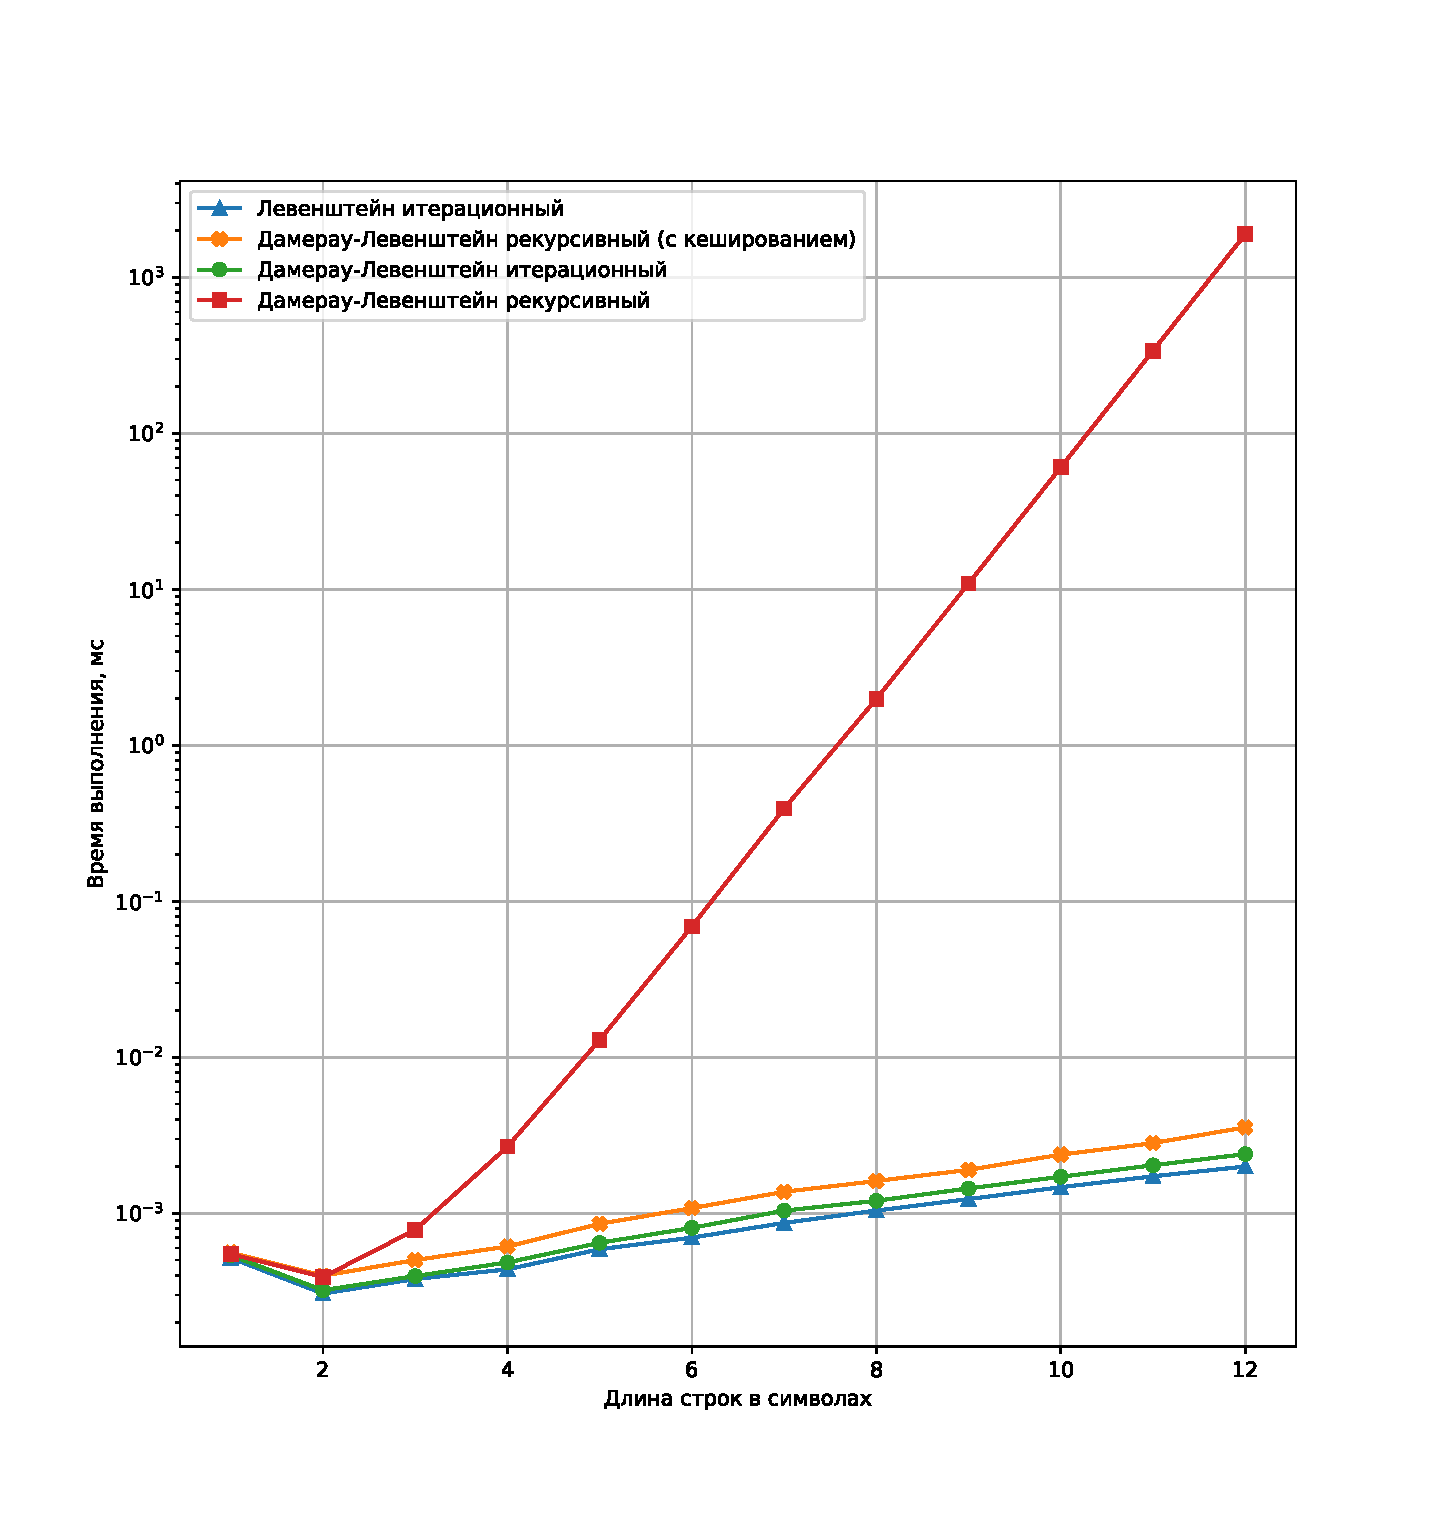
\includegraphics[width=\textwidth]{img/fn_four.pdf}
	\caption{Сравнение всех реализаций алгоритмов по времени выполнения (среднее время из 10 замеров)}
	\label{fig:fn_four}
\end{figure}

% \begin{figure}[H]
% 	\centering
% 	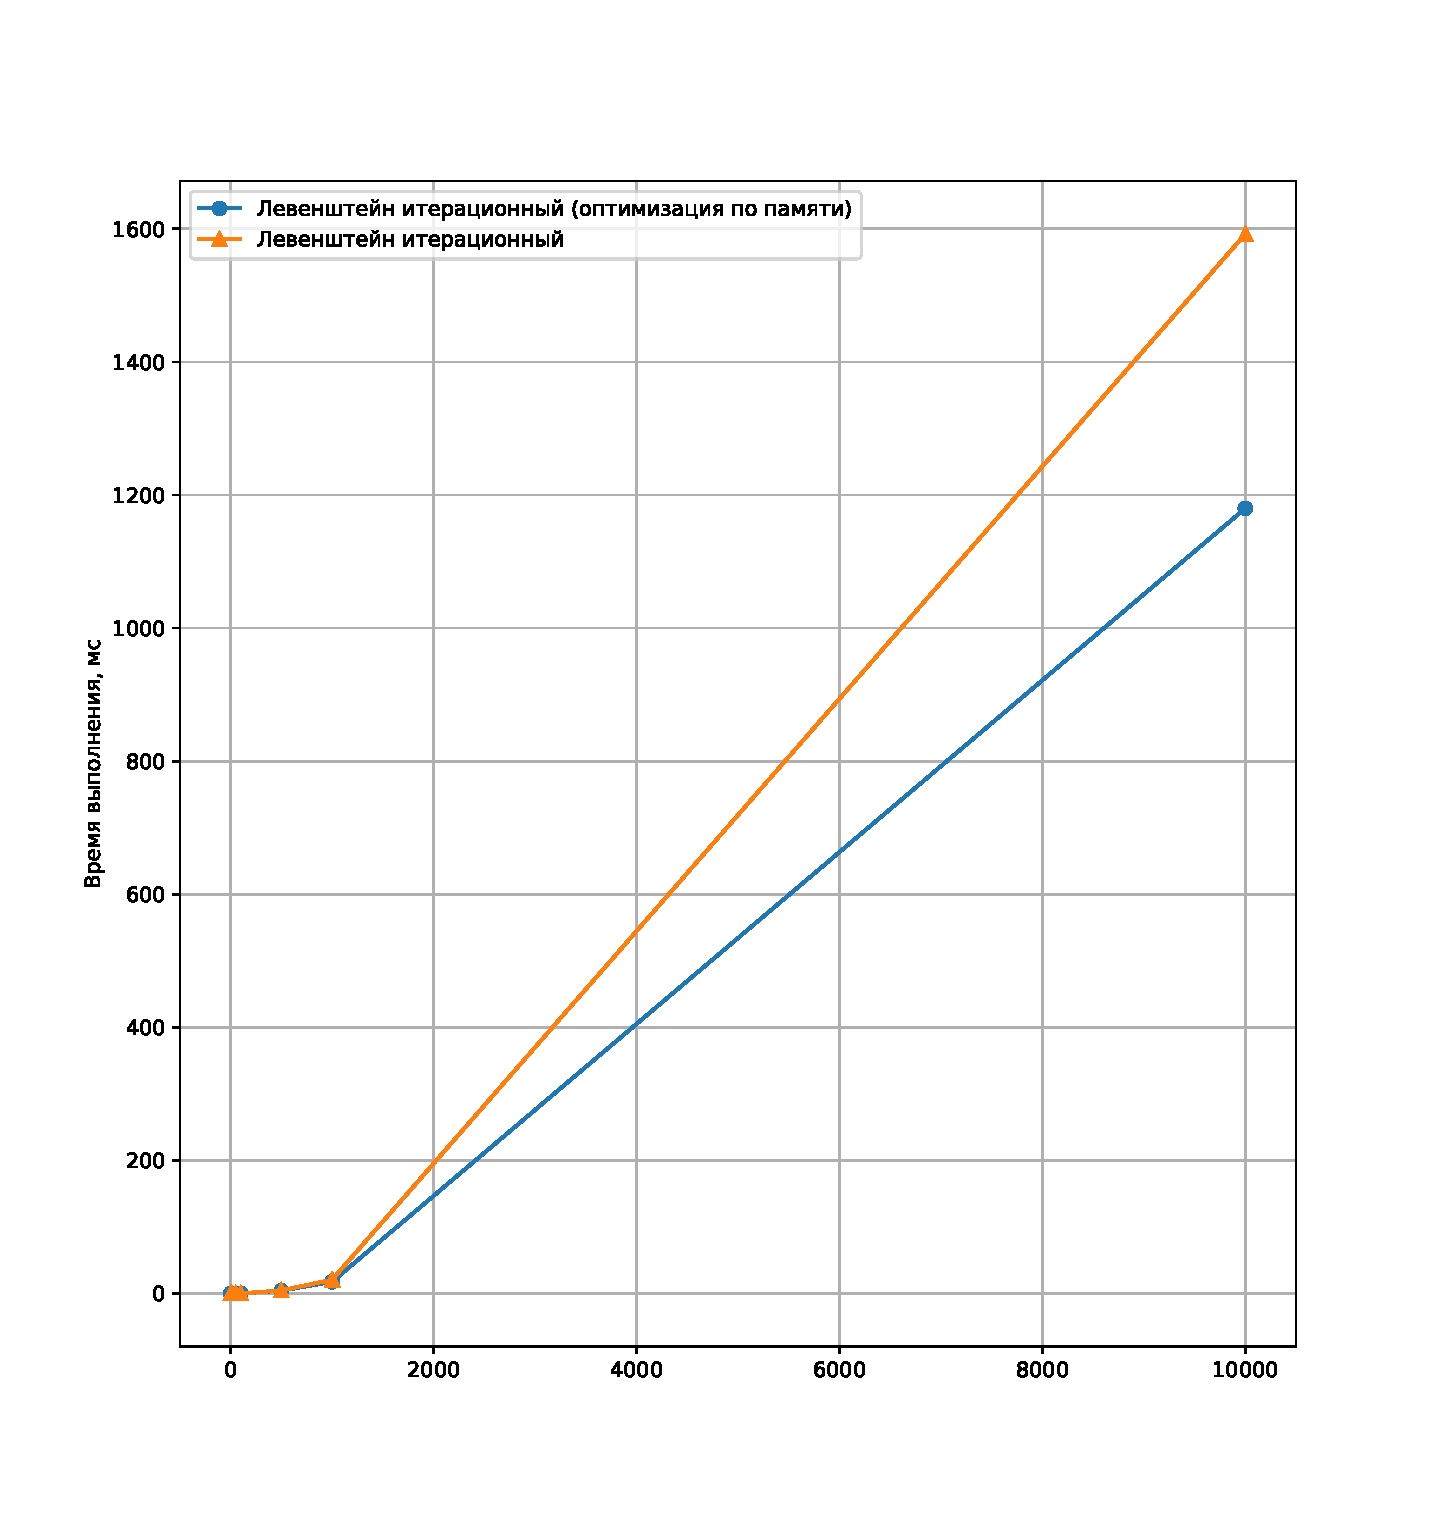
\includegraphics[width=\textwidth]{img/fn_lev_10k_time.pdf}
% 	\caption{}
% 	\label{fig:fn}
% \end{figure}

\newpage

\subsection{Теоретические оценки затрачиваемой памяти}

Введём следующие обозначения:
\begin{itemize}
    \item $L_1$ --- длина первой строки;
    \item $L_2$ --- длина второй строки;
    \item $char$ --- символьный тип данных;
    \item $*$ --- тип данных --- указатель;
    \item $int$ --- целочисленный тип данных;
    \item $size()$ --- функция, вычисляющая размер типа данных в байтах, т.е. на практике $size(char) \sim sizeof(wchar\_t)$;
\end{itemize}

На основе введённых обозначений проведём теоретическую оценку памяти, используемой реализациями алгоритмов.

\subsubsection{Оценка памяти реализаций итерационных алгоритмов нахождения расстояний Левенштейна и Дамерау --- Левенштейна}
\begin{itemize}
    \item Первая строка: $L_1 \cdot size(char)$;
    \item Вторая строка: $L_2 \cdot size(char)$;
    \item Размеры строк: $2 \cdot size(int)$;
    \item Указатели на строки и адрес возврата: $3 \cdot size(*)$;
    \item Матрица: $(L_1 + 1) \cdot (L_2 + 1) \cdot size(int) + (L_1 + 1) \cdot size(*) + size(*)$;
    \item Вспомогательные переменные: $c \cdot size(int)$, где $c$ --- количество вспомогательных переменных;
\end{itemize}

Итого, функция суммарного объёма используемой памяти, имеет вид:
\begin{multline}
\begin{aligned}
V(L_1,L_2) =\ &L_1 \cdot size(char) + L_2 \cdot size(char) \\
&+ 2 \cdot size(int) + (L_1 + 1) \cdot (L_2 + 1) \cdot size(int) \\
&+ 3 \cdot size(*) + (L_1 + 1) \cdot size(*) + size(*) + c \cdot size(int)
\end{aligned}
\end{multline}

Просуммировав все значения и приняв $size(\dots)$ за константы, можно сделать вывод, что $V(L_1,L_2) \in \Theta(L_1 \cdot L_2)$.

\subsubsection{Оценка памяти реализации рекурсивного алгоритма нахождения расстояния Дамерау --- Левенштейна}
\begin{itemize}
    \item Первая строка: $L_1 \cdot size(char)$;
    \item Вторая строка: $L_2 \cdot size(char)$;
    \item Размеры строк: $2 \cdot size(int)$;
    \item Указатели на строки и адрес возврата: $3 \cdot size(*)$;
    \item Вспомогательные переменные: $c \cdot size(int)$, где $c$ --- количество вспомогательных переменных;
\end{itemize}

Максимальная глубина стека вызовов при рекурсивной реализации алгоритма нахождения расстояния Дамерау --- Левенштейна равна сумме длин входящих строк, соответственно, максимальный расход памяти рассчитывается по:
\begin{multline}
\begin{aligned}
V(L_1,L_2) =\ &(L_1 + L_2) \cdot ((2 + c) \cdot size(int) + 3 \cdot size(*))
\end{aligned}
\end{multline}

Просуммировав все значения и приняв $size(\dots)$ за константы, можно сделать вывод, что $V(L_1,L_2) \in \Theta(L_1 + L_2) = \Theta(L)$, то есть, максимальный расход памяти линейно зависит от длины входящих строк.

\subsubsection{Оценка памяти реализации рекурсивного с кешированием алгоритма нахождения расстояния Дамерау --- Левенштейна}

\begin{itemize}
    \item Первая строка: $L_1 \cdot size(char)$;
    \item Вторая строка: $L_2 \cdot size(char)$;
    \item Размеры строк: $2 \cdot size(int)$;
    \item Указатели на строки и адрес возврата: $3 \cdot size(*)$;
    \item Матрица: $L_1 \cdot L_2 \cdot size(int) + L_1 \cdot size(*) + size(*)$;
    \item Вспомогательные переменные: $c \cdot size(int)$, где $c$ --- количество вспомогательных переменных;
\end{itemize}

Итого, под матрицу используется:
\begin{multline}
\begin{aligned}
V_M(L_1,L_2) =\ &L_1 \cdot L_2 \cdot size(int) + L_1 \cdot size(*) + size(*) \in \Theta(L_1 \cdot L_2)
\end{aligned}
\end{multline}

Под стек будет использоваться меньше памяти, чем в исключительно рекурсивной реализации, так как функция не будет углублять стек вызовов, если встретится уже вычисленное ранее значение.
Следовательно, $V_S(L_1,L_2) \in \Theta(L)$.

Тогда суммарный объём используемой памяти имеет вид:
\begin{multline}
\begin{aligned}
V(L_1,L_2) = V_M(L_1,L_2) + V_S(L_1,L_2) \in \Theta(L_1 \cdot L_2) + \Theta(L) = \Theta(L_1 \cdot L_2)
\end{aligned}
\end{multline}

Таким образом, рекурсивная без кеширования реализация алгоритма нахождения Дамерау --- Левенштейна расходует меньше памяти при достаточно длинных строках по сравнению с остальными реализациями.
Её расход памяти растёт пропорционально $L_1 + L_2$, в то время как расход памяти остальных реализаций алгоритмов растёт пропорционально $L_1 \cdot L_2$.

\subsection{Характеристики по памяти}

На графиках \ref{fig:fn_rec_calls} -- \ref{fig:fn_iter_heap} представлены результаты измерения затрачиваемой памяти реализациями алгоритмов нахождения расстояний Левенштейна и Дамерау~---~Левенштейна.
Замеры памяти проводились для строк одинаковой длины.
Отображённая на графиках память является усреднённой для каждой длины строк.

\begin{figure}[H]
	\centering
	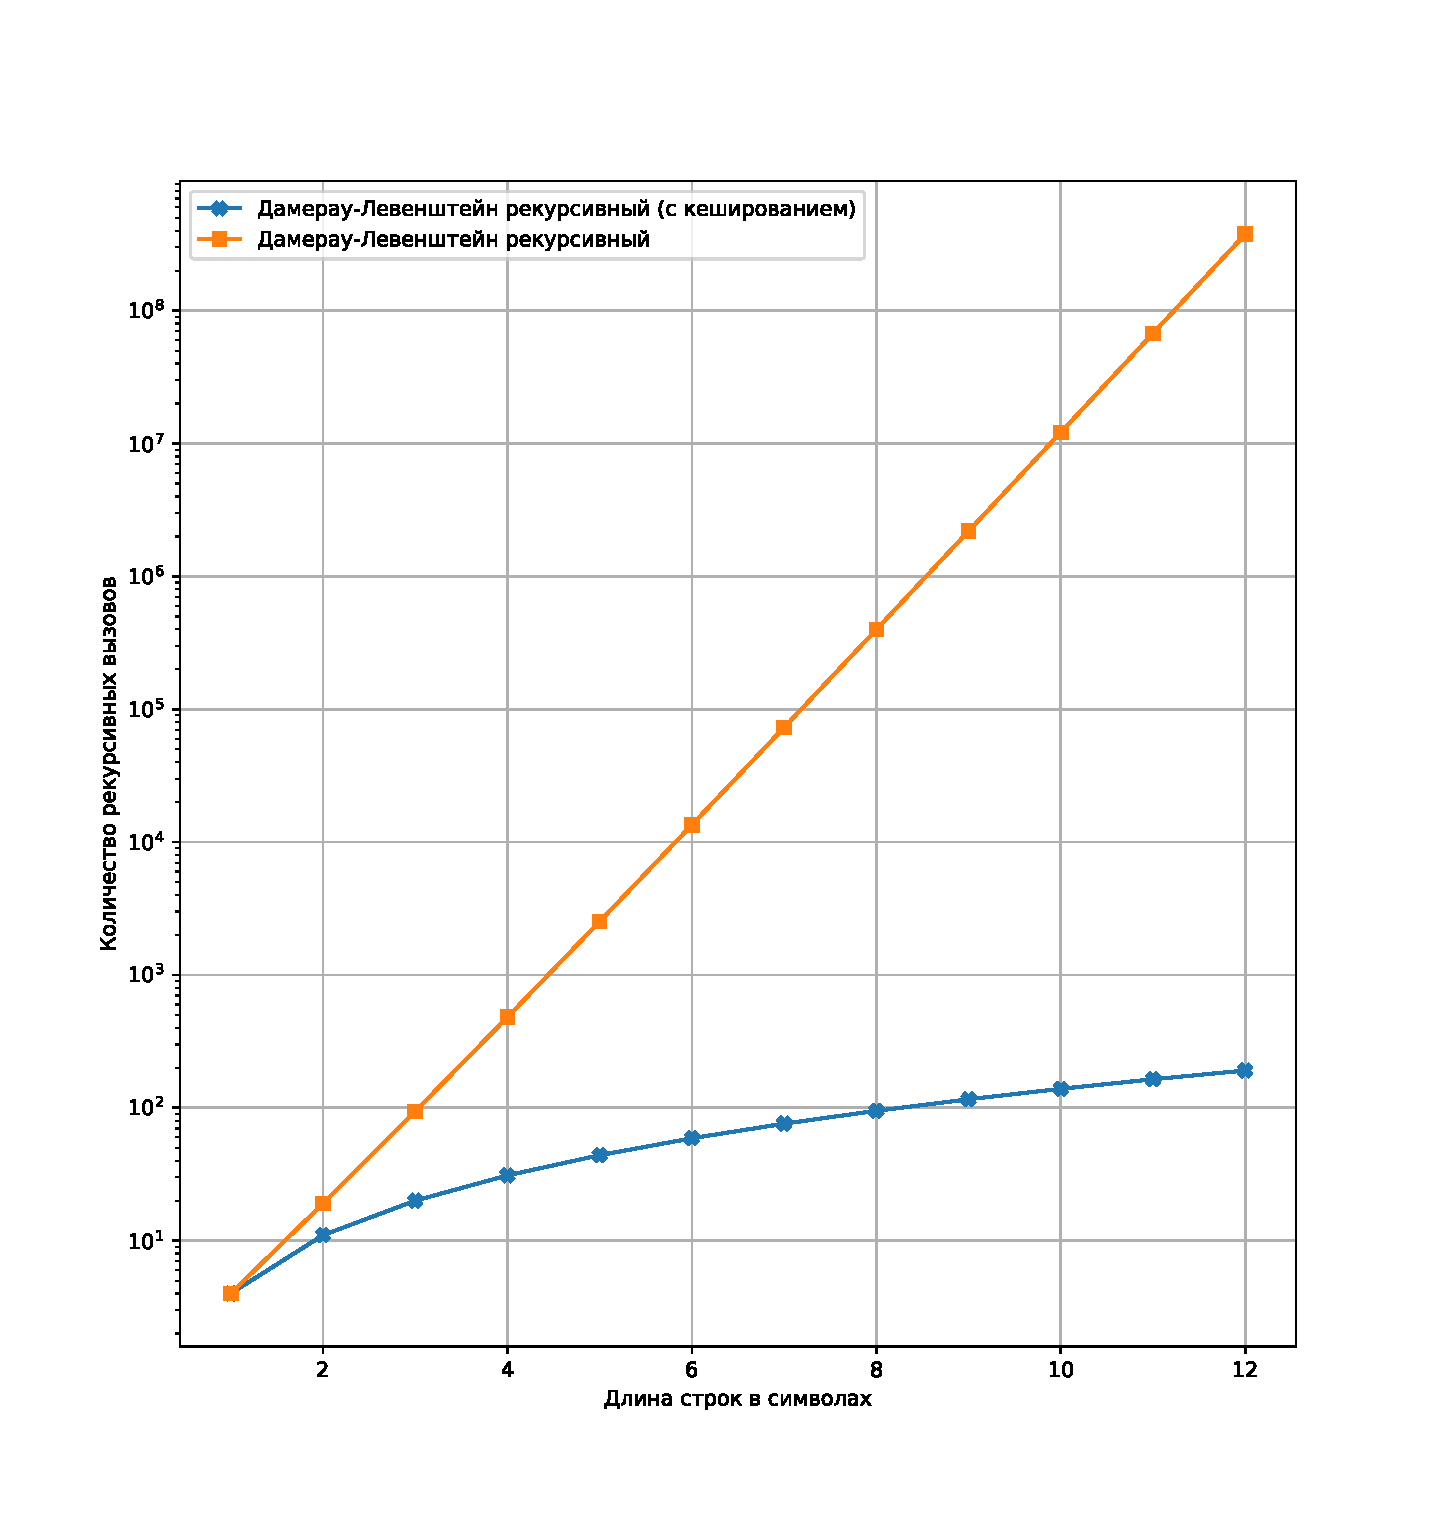
\includegraphics[width=\textwidth]{img/fn_rec_calls.pdf}
	\caption{Сравнение количества рекурсивных вызовов у рекурсивных реализаций алгоритмов нахождения расстояния Дамерау~---~Левенштейна}
	\label{fig:fn_rec_calls}
\end{figure}

\begin{figure}[H]
	\centering
	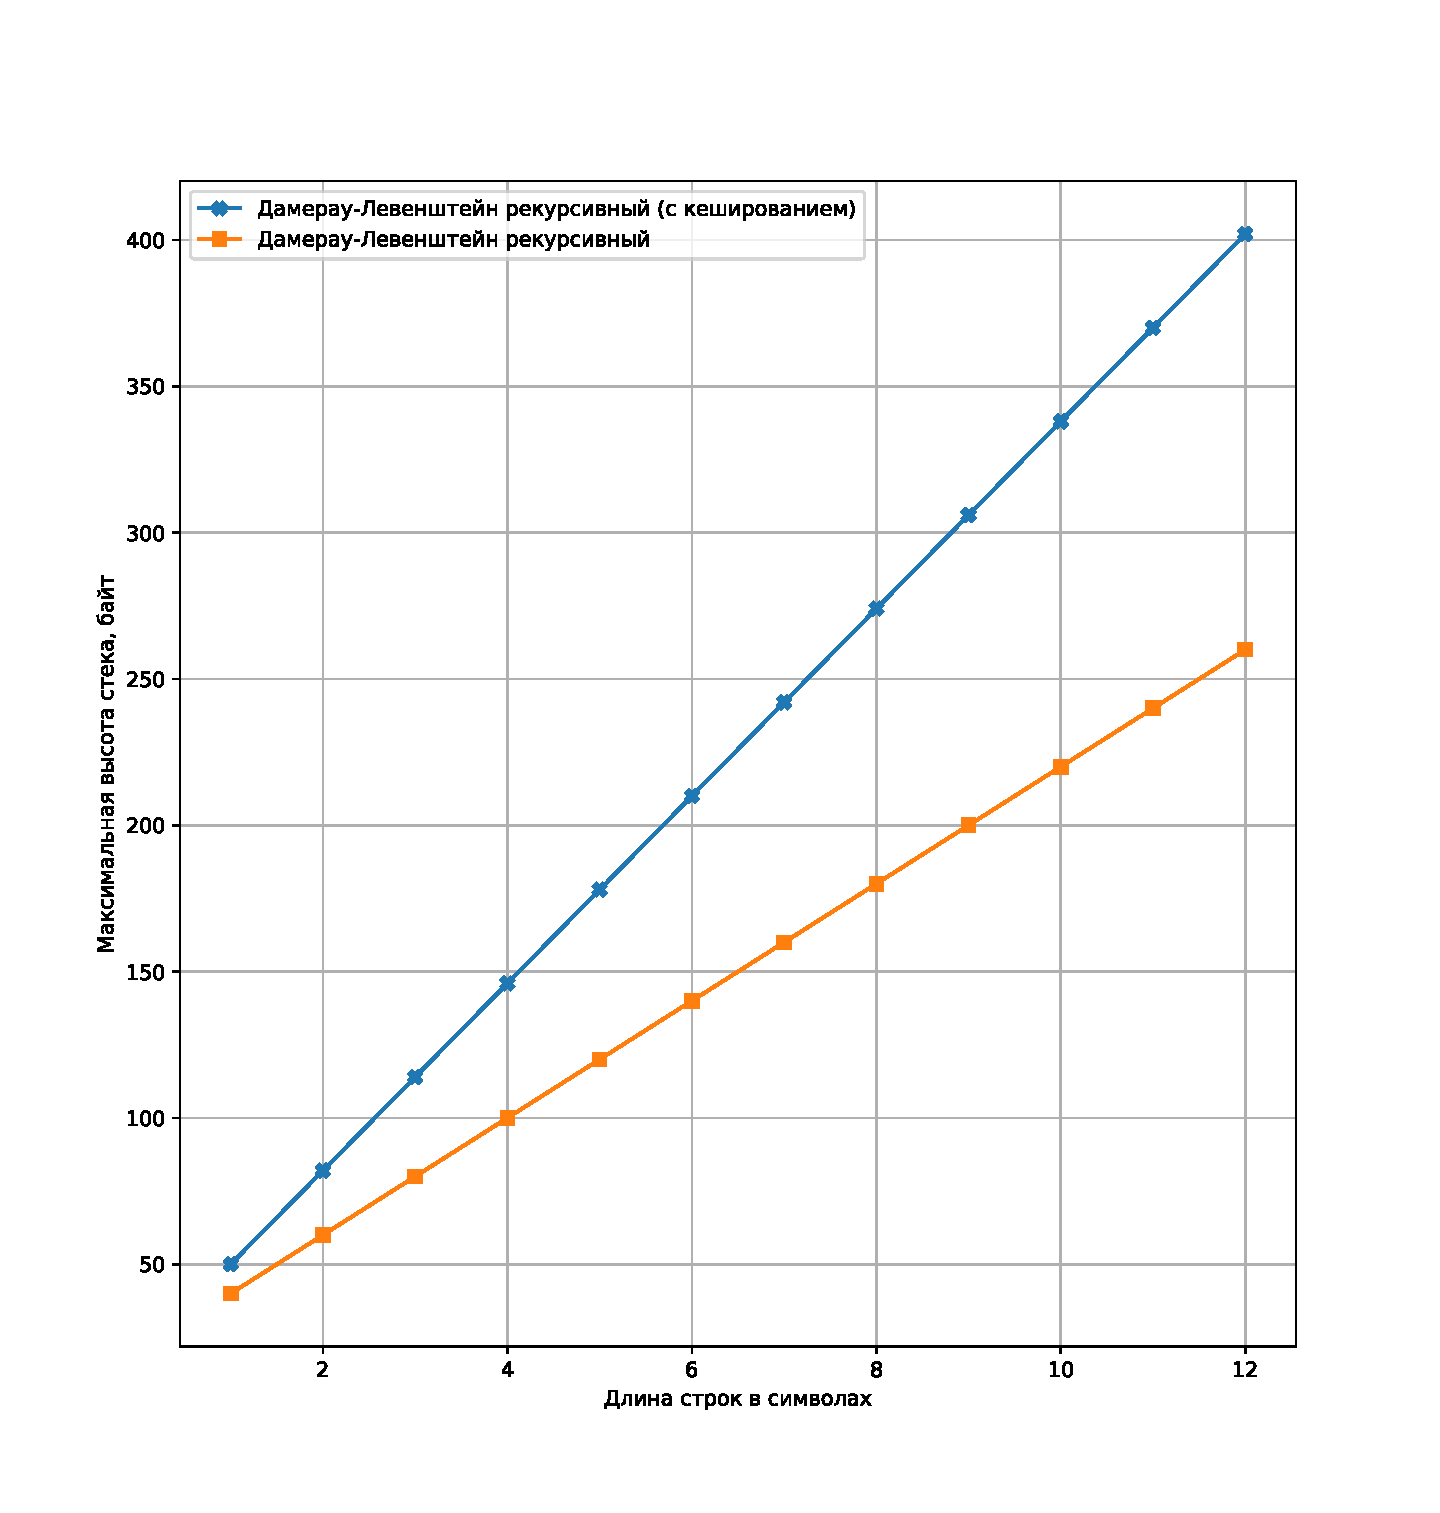
\includegraphics[width=\textwidth]{img/fn_max_stack.pdf}
	\caption{Сравнение максимальной высоты стека вызовов у рекурсивных реализаций алгоритмов нахождения расстояния Дамерау~---~Левенштейна}
	\label{fig:fn_max_stack}
\end{figure}

\begin{figure}[H]
	\centering
	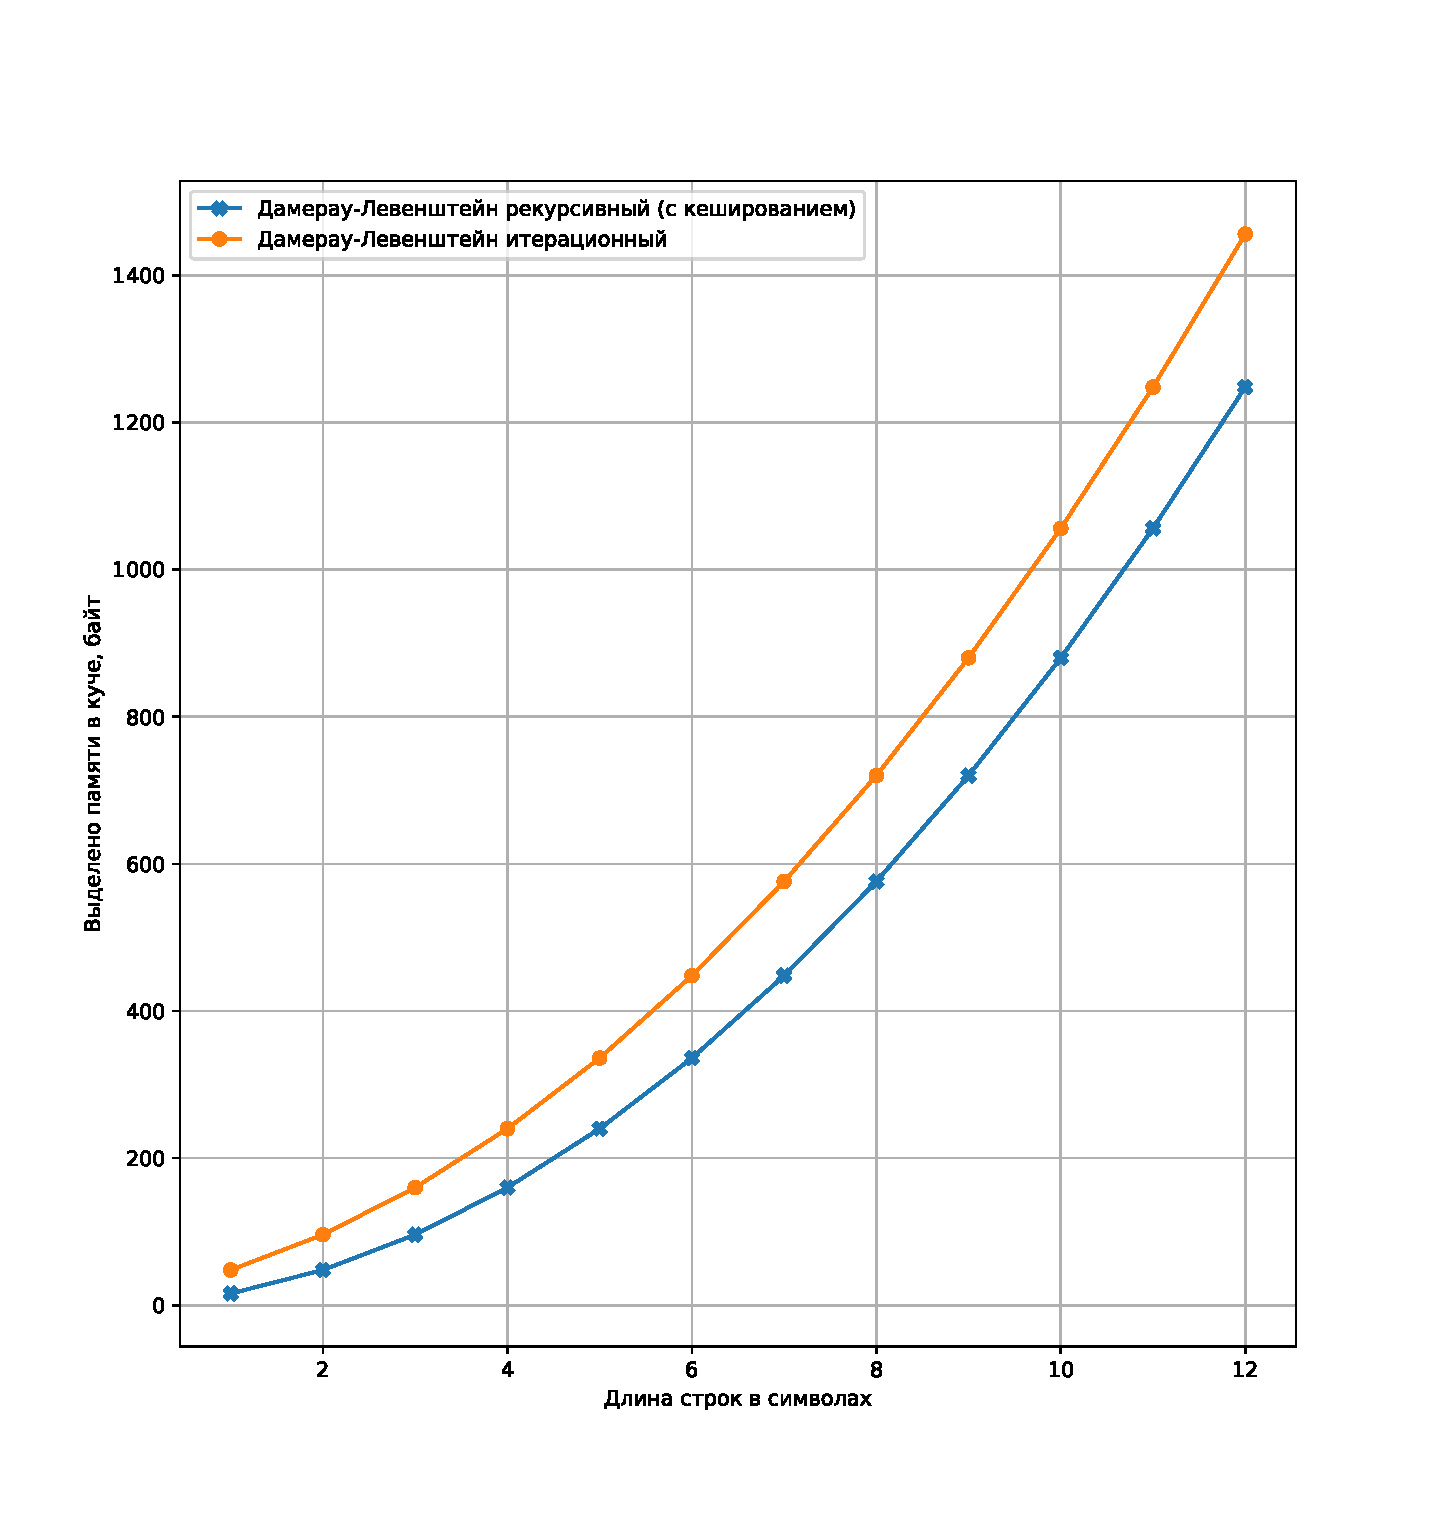
\includegraphics[width=\textwidth]{img/fn_heap.pdf}
	\caption{Сравнение выделяемой памяти в куче для итерационного и рекурсивного с кешированием реализаций алгоритмов нахождения расстояния Дамерау~---~Левенштейна}
	\label{fig:fn_heap}
\end{figure}

\begin{figure}[H]
	\centering
	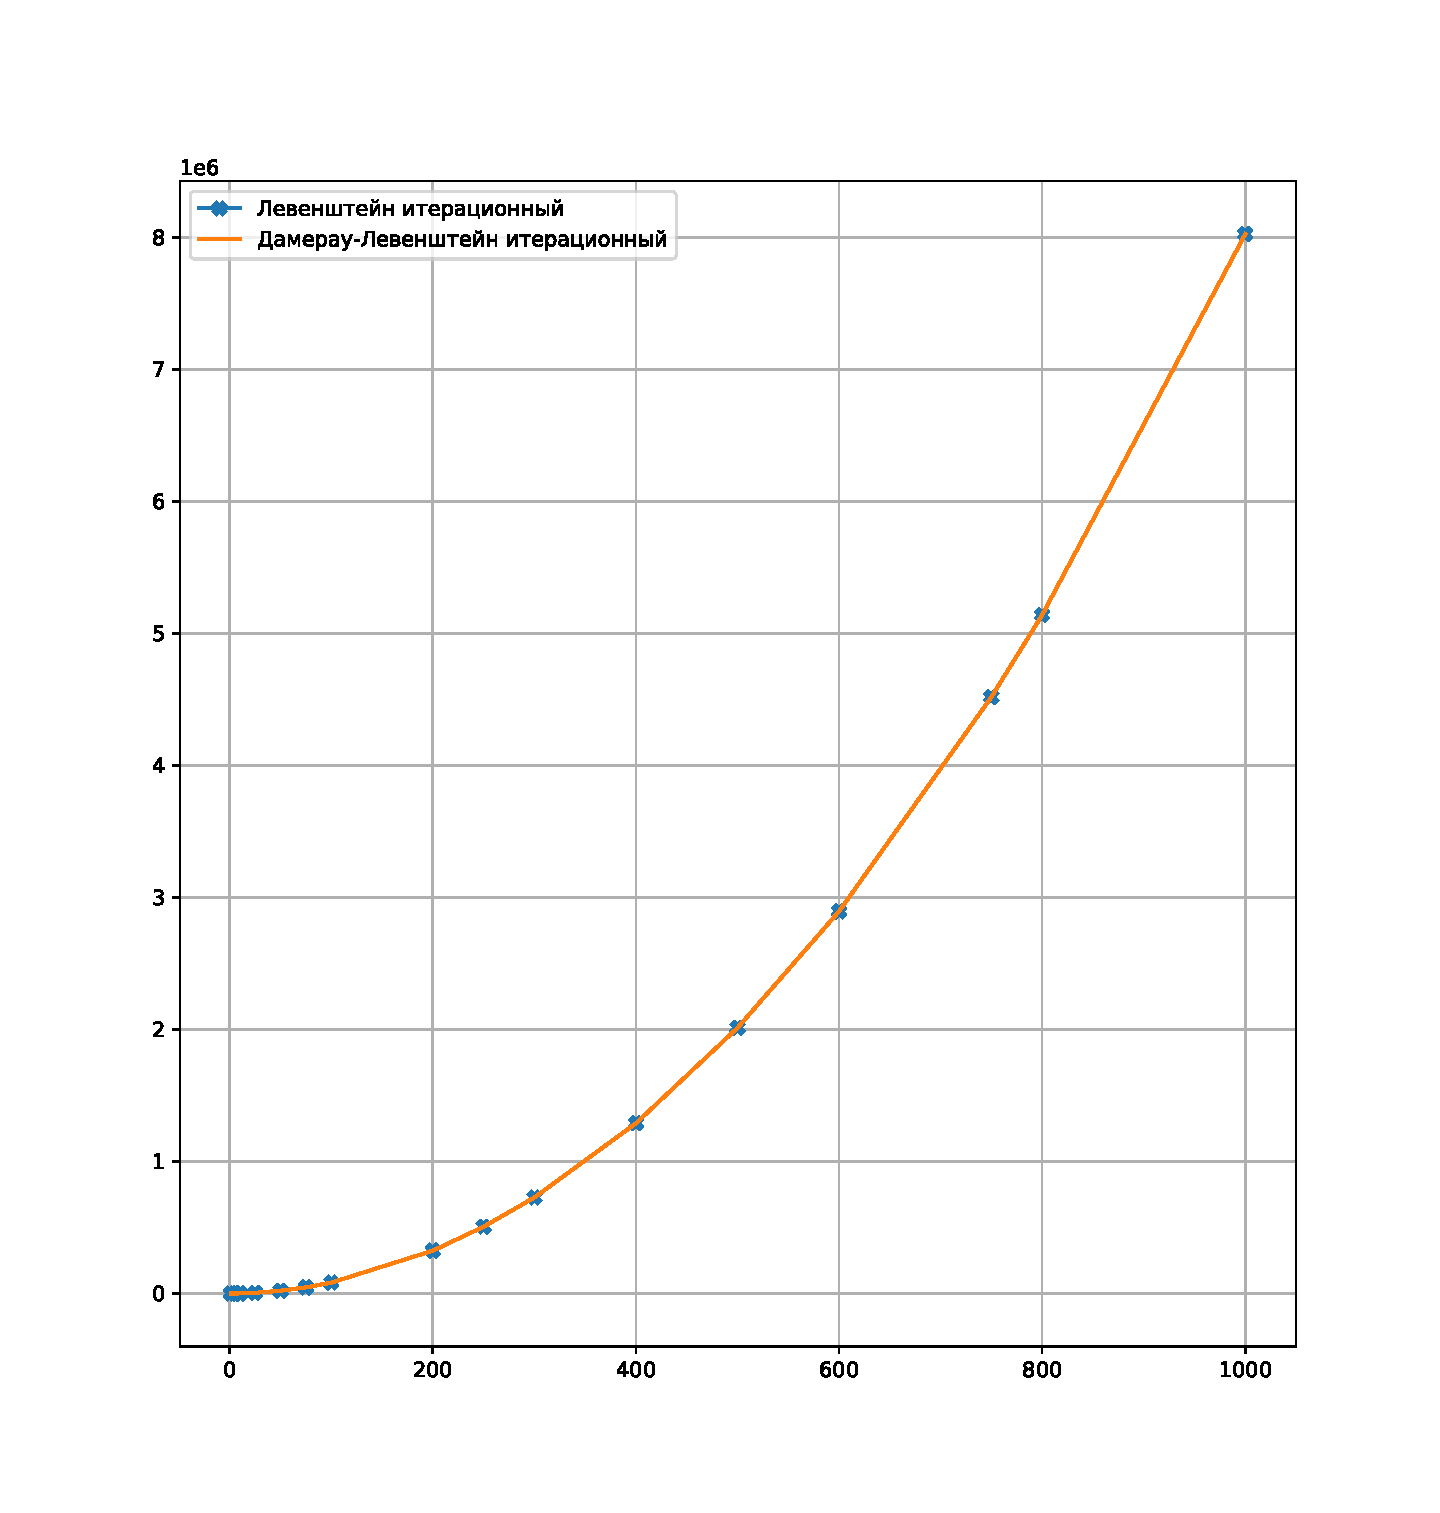
\includegraphics[width=\textwidth]{img/fn_iter_heap.pdf}
	\caption{Сравнение выделяемой памяти в куче для итерационных реализаций алгоритмов нахождения расстояний Левенштейна и Дамерау~---~Левенштейна}
	\label{fig:fn_iter_heap}
\end{figure}

% \begin{figure}[H]
% 	\centering
% 	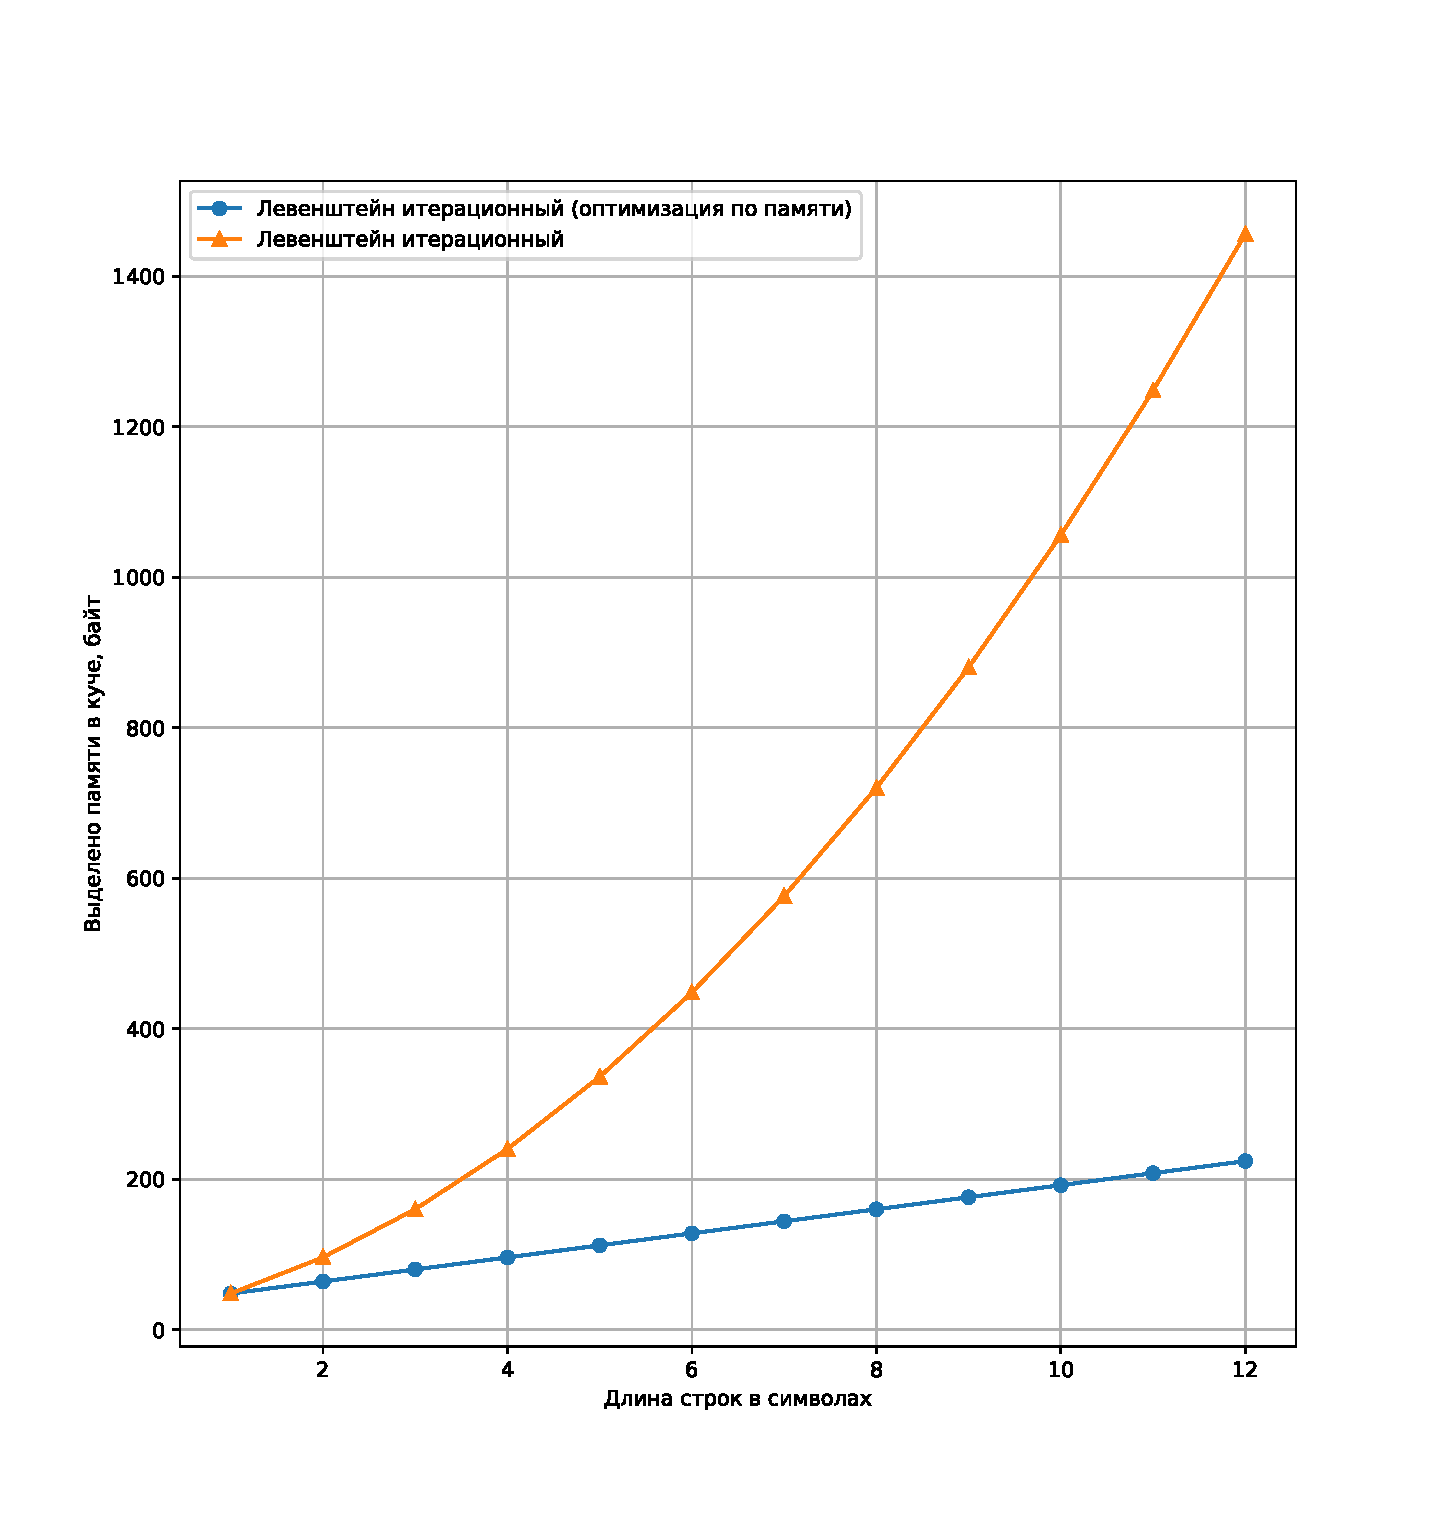
\includegraphics[width=\textwidth]{img/fn_mem_lev_optimized.pdf}
% 	\caption{}
% 	\label{fig:fn}
% \end{figure}

\newpage

\subsection*{Вывод}

В данном разделе было произведено сравнение количества затраченного времени и памяти реализаций алгоритмов поиска расстояний Левенштейна и Дамерау --- Левенштейна. Наименее затратной по времени оказалась итерационная реализация алгоритма нахождения расстояния Левенштейна.

Проанализировав использование памяти в алгоритмах, можно сделать вывод, что итеративные алгоритмы и рекурсивные алгоритмы с кешированием требуют больше памяти по сравнению с рекурсивным алгоритмом без кеширования.
В реализациях, использующих матрицы, максимальный используемый объем памяти увеличивается пропорционально произведению длин строк.
С другой стороны, для рекурсивного алгоритма без кеширования потребление памяти увеличивается пропорционально сумме длин строк.
